\chapter{Diseño Electromecánico} \label{chap:Electronica}
\hrule
\vspace{3mm}
En este capítulo se hará una descripción detallada de todos los componentes involucrados en el proyecto.

\section{Actuadores} \label{sec:Electronica:Actuadores}
\label{sec:Electronica:Actuadores:G15}

    Para los grados de libertad de posición del prototipo se ha optado por utilizar los \glosarioPlural{smartservo} G15 Cube de la marca Cytron.
    
    Algunas características importantes de los mismos se muestran en la tabla \ref{tab:g15_catact}:
    
    \begin{table}[H]
    	\caption{Características mas importantes de los Servos G15 de Cytron. Tabla traducida y resumida a los puntos más importantes del Cytron G15 Cube servo User Manual \cite{CytronTechnologies2012} \completarCon{¿esto está bien, hay que poner paginas involucradas?}}
    	\label{tab:g15_catact}
   		\begin{minipage}{0.42\textwidth}
   		\begin{center}
   		\begin{tabular}{ |c|c|c|c| }
			\hline
			\multicolumn{4}{|c|}{\textbf{Características eléctricas}} \\ 
			\hline
			\textbf{Parámetro} & \textbf{Valor Mínimo} & \textbf{Valor Típico} & \textbf{Valor Máximo} \\
			\hline
			Voltaje & $6.5V$ & $12V$ & $17.8V$ \\
			\hline
			Consumo de corriente ($12V$) & & & $1.5A$ \\
			\hline
			Temperatura de funcionamiento & $0^oC$ & & $80^oC$ \\
			\hline
			Par capaz de soportar & & & $15km \cdot cm$ \\
			\hline
			\multicolumn{4}{c}{\textbf{}} \\ 
			\hline
			\multicolumn{4}{|c|}{\textbf{Especificaciones técnicas}} \\ 
			\hline
			\multicolumn{2}{|c|}{Peso} & \multicolumn{2}{|c|}{$63g$}\\ 
			\hline
			\multicolumn{2}{|c|}{Par capaz de realizar (a $12V$)} & \multicolumn{2}{|c|}{$12kg \cdot cm$}\\ 
			\hline
			\multicolumn{2}{|c|}{Margen angular de operación } & \multicolumn{2}{|c|}{$360^o$ en giro continuo}\\ 
			\hline
			\multicolumn{2}{|c|}{Máxima velocidad (en vacío a $12V$)} & \multicolumn{2}{|c|}{$63 RPM$ }\\ 
			\hline    			
			\multicolumn{2}{|c|}{Comunicaciçon} & \multicolumn{2}{|c|}{ \begin{minipage}{1.0\textwidth}\vspace{0.1cm}
			Half duplex asynchronous serial \\ communication ($7812.5bps-500kbps $)\end{minipage} }\\ 
    		\hline    				 	 
    	\end{tabular}
   		\end{center}
   		\end{minipage}
    \end{table}
    
	Estos servos utilizan un protocolo de comunicación basado en una comunicación \ingles{Half Duplex Serial}. En este caso toda la información fluye por un mismo cable. Los servos se conectan en un bus uno a continuación del otro, teniendo tres pines, uno de voltaje positivo, otro de GND y el tercero de datos. Se puede ver en la figura \ref{fig:Electronica:bus-servos} como quedan conectados a la placa, quedando uno de los extremos (el del último servo) libre.
    \begin{figure}[H]
    	\centering
    	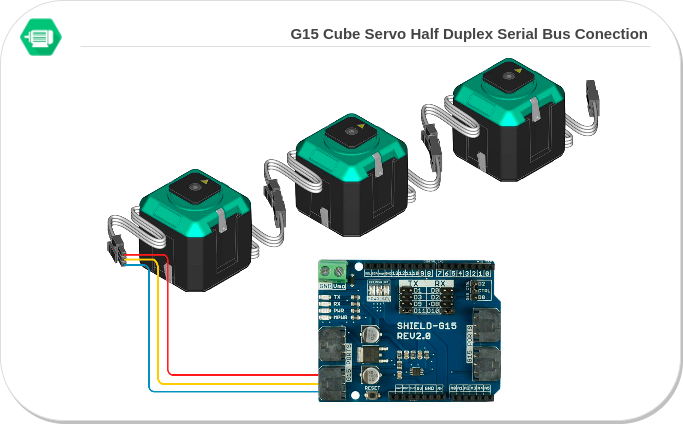
\includegraphics[width=0.9\textwidth]{figuras/Imagenes_Electronica/G15_bus_conection.png}   
    	\caption{Esquema de la conexión el bus serie de servos y la placa Shield}
    	\label{fig:Electronica:bus-servos}
    \end{figure}

\section{Etapa de potencia} \label{sec:Electronica:Potencia}

	Para la correcta comunicación entre los servos y la placa se utilizan tres pines de la misma. Dos serán los de entrada (RX) y salida (TX) para comunicar y el tercer pin funcionará a modo de pin de control, gestionando en que momentos se publica información por el pin de salida y en que momento se escucha por el pin de entrada.
	\\
	
	Dependiendo de que placa se utilice este puerto serie (el TX y el RX) podrán estar conectados a un puerto serie de tipo Hardware o emular uno por Software. 
	\\
	
	En primeras versiones del desarrollo se ha estado utilizando un Arduino Uno en el cual se emulaba, por los pines 9 (TX) y 8 (RX) un puerto software quedando el puerto Hardware de los pines 1 y 0 para la comunicación serie con el ordenador.
	\\
	
	Debido a los ciclos de funcionamiento del software para aplicar el control al brazo robótico esta comunicación resulta ser demasiado lenta, es por ello que se sustituye el Arduino Uno por un Arduino Mega, con 4 puertos serie Hardware que se podrán aprovechar, para la comunicación con el ordenador (pines 0 y 1) y para la comunicación con los servos (pines 18 y 19).
	\\ 
	
	En la Shield utilizada para comunicar con los servos viene preparado para, mediante unos jumpers \completarCon{definir?¿}, poder seleccionar unos pines u otros. En este caso no está preparado para comunicar con un Arduino Mega directamente, es por ello que se han sacado unos cables para conectar, la parte de la shield que conecta con el puerto de los servos (están los 4 pines cortocircuitados) con los pines de los puertos hardware del Arduino Mega. Se puede ver dicha conexión en la figura \ref{fig:Electronica:shield-arduino}.
	
    \begin{figure}[H]
    	\centering
    	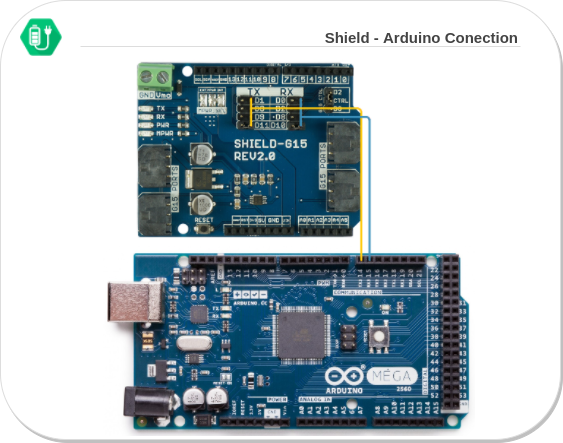
\includegraphics[width=0.65\textwidth]{figuras/Imagenes_Electronica/Shield-Arduino-Conection.png}   
    	\caption{Esquema de la conexión entre la placa Shield y Arduino para utilizar los puertos Hardware Serie de la Arduino Mega}
    	\label{fig:Electronica:shield-arduino}
    \end{figure}
\section{Procesamiento}

\section{Sensores} \label{sec:Electronica:Sensores}



